% !TEX encoding = UTF-8 Unicode

\documentclass{article}
\usepackage[french]{babel}
\author{Louis DESVERNOIS}
\title{Procédure d'installation et de déploiement pour la SAÉ23.}
% \date{9 Juin 2022}
\usepackage[margin=1in]{geometry}
\usepackage{subcaption}
\usepackage{listings}
\usepackage{minted}
\usepackage{graphicx}
\usepackage[T1]{fontenc}
\usepackage[colorlinks=true,linkcolor=black,anchorcolor=black,citecolor=black,filecolor=black,menucolor=black,runcolor=black,urlcolor=black]{hyperref}
%\setcounter{tocdepth}{1} % Show sections
%\setcounter{tocdepth}{2} % + sections
%\setcounter{tocdepth}{3} % + subsections
%\setcounter{tocdepth}{4} % + paragraphs
%\setcounter{tocdepth}{5} % + subparagraphs
%\renewcommand{\contentsname}{Tables des matières} % Change le nom de la ToC
%\renewcommand{\listfigurename}{Liste des figures}

\renewcommand{\listoflistingscaption}{Table des codes}
\renewcommand{\listingscaption}{Code}
% \renewcommand{\bibname}{Bibliographie} % Change le nom des références (bibname pour les classes book et report)

\begin{document}

\maketitle
\tableofcontents
\listoffigures
\listoflistings
\newpage
\section{Machine virtuelle et base de données}
    Notre solution se base sur une machine virtuelle utilisant la dernière version de Debian 11. La technologie utilisée pour créer cette machine virtuelle n'a peu d'importance, tant que celle-ci est accessible (e.g., carte réseau en mode bridge). 

        \subsection{Installations des dépendances}
        Après l'installation d'un système minimal Debian 11, nous avons besoin d'installer les différents composant nécessaire au déploiement d'un serveur MariaDB ainsi qu'un serveur HTTP nginx.
        \begin{listing}[H]
            \begin{minted}[breaklines]{bash}
apt install git mariadb-server nginx python3 python3-pip python3-venv python3-dev libmariadb-dev ufw -y
            \end{minted}
            \caption{Installation des dépendances}
            \label{code:deps-install}
        \end{listing}

        \subsection{Configuration initiale de la base de données}
        En installant le paquet \verb|mariadb-server|, le gestionnaire de paquets apt a déjà automatique activé le service. Il nous reste donc qu'à configurer le serveur.
        \begin{listing}[H]
            \begin{minted}[breaklines]{sql}
mysql -sfu root <<EOS
UPDATE mysql.user SET Password=PASSWORD('toto') WHERE User='root';
DELETE FROM mysql.user WHERE User='';
DROP DATABASE IF EXISTS test;
DELETE FROM mysql.db WHERE Db='test' OR Db='test\\_%';
FLUSH PRIVILEGES;
CREATE USER 'toto'@'localhost';
EOS
            \end{minted}
            \caption{Configuration initiale du serveur MariaDB}
            \label{code:initdbconf}
        \end{listing}
        Pour la configuration, nous utilisons la commande \verb|mysql -sfu root| pour nous connecter à la base de données et ignorer les erreurs (Code \ref{code:initdbconf}). Pour commencer, nous changeons le mot de passe de l'utilisateur "root", nous supprimons tous les utilisateurs anonymes, nous supprimons la base de données "test" si elle existe, puis nous créons l'utilisateur "toto", qui permettra à Django d'accéder à la base de données.

        \subsection{Création de l'utilisateur, clonage du dépôt GitHub et exécution du script SQL}
        Pour des raisons de sécurité, est préférable de ne pas exécuter le code python de notre site avec le super-utilisateur, c'est pour cela que nous créons un utilisateur ainsi que son dossier personnel sur notre serveur. 
        \begin{listing}[H]
            \begin{minted}[breaklines]{bash}
useradd -m toto
su - toto -c "git clone https://github.com/ldsvrn/SAE23-TraficAerien /home/toto/django"
            \end{minted}
            \caption{Création de l'utilisateur et clonage du dépôt GitHub}
            \label{code:newutil}
        \end{listing}
        Après la création de l'utilisateur avec la commande \verb|useradd -m|, nous pouvons cloner le dépôt avec la commande \verb|git clone <url> <dst>|
        \footnote{\label{note1}"su - toto -c" est utilisé dans le code \ref{code:newutil} pour exécuter la commande avec l'utilisateur toto}.

        \begin{listing}[H]
            \begin{minted}[breaklines]{bash}
mysql -u root -p'toto' < /home/toto/django/SAE_23_BDD.sql
mysql -sfu root -p'toto'<<EOS
-- permission d'acces à la base de donnée
GRANT ALL PRIVILEGES ON sae_23.* TO 'toto'@'localhost';
EOS
            \end{minted}
            \caption{Importation de notre script SQL}
            \label{code:execsql}
        \end{listing}
        Ensuite, nous pouvons utiliser les commandes ci-dessus (\ref{code:execsql}) pour importer notre script SQL préalablement téléchargé lors du \verb|git clone| exécuté précédemment (Code \ref{code:newutil}). Nous octroyons ensuite à l'utilisateur "toto" tous les droits sur la base de données importée.

\section{Environnement virtuel Python}
    Pour faire fonctionner Django, nous allons avoir besoin d'un environnement virtuel (venv) pour installer Django et ses dépendances sans les installer pour tout le système. Travailler avec des venv permet de garantir que paquets installés soient toujours les mêmes. 

        \subsection{Création de l'environnement et installation des paquets}
        Le module \verb|venv| de Python nous permet de créer ces environnements facilement avec la commande \verb|python -m venv .venv|.
        En supposant que l'on utilise le shell bash, nous pouvons ensuite activer cet environnement grâce à la commande \verb|source|.
        Une fois l'environnement virtuel activé, nous pouvons simplement utiliser \verb|pip3| pour installer les dépendances de notre projet
        \footnote{\label{note2}Il est également possible d'utiliser le fichier requirements.txt avec la commande "pip3 install -r requirements.txt"}. 
        Nous pouvons donc exécuter les commandes suivantes, cette fois ci avec l'utilisateur créé précédemment (Code \ref{code:newutil}). 
        \begin{listing}[H]
            \begin{minted}{bash}
python -m venv .venv
source .venv/bin/activate
pip3 install django django-admin mysqlclient gunicorn crispy-bootstrap5 Pillow reportlab
            \end{minted}
            \caption{Création du venv et installation des paquets}
            \label{code:creation-venv}
        \end{listing}
        
        \subsection{Configuration du projet Django (settings.py)}
        Une fois toutes dépendances python installées dans l'environnement virtuel, nous devons modifier les paramètres de notre projet Django afin d'utiliser la base de données externe.
        Il est intéressant de vérifier si le répertoire des fichiers statiques (e.g., images, css) est correctement configuré
        \footnote{\label{note3}Normalement, cela est déjà configuré automatiquement à la création du projet}. 
        \begin{listing}[H]
            \begin{minted}{python}
DATABASES = {
    'default': {
        'ENGINE': 'django.db.backends.mysql',
        'NAME': 'sae_23',
        'USER': 'toto',
        'PASSWORD': '',
        'HOST': 'localhost',
        'PORT': '3306',
    }
}
            \end{minted}
            \caption{settings.py : Paramétrages de la base de données}
            \label{code:settings.py-db}
        \end{listing}
        
        \subsection{Préparation du projet au déploiement}
        Avant de commencer à mettre en place notre serveur web, nous avons besoin de préparer notre projet au déploiement.
        Pour cela nous devons utiliser le fichier \verb|manage.py| pour préparer la base de données ainsi que les fichiers statiques. En nous plaçant à la racine de notre projet, nous pouvons exécuter les commandes suivantes
        \footnote{Commandes à exécuter avec l'utilisateur crée en Code \ref{code:newutil}}.
        \begin{listing}[H]
            \begin{minted}{bash}
python3 manage.py makemigration
python3 manage.py migrate
python3 manage.py collectstatic
            \end{minted}
            \caption{Préparation de la base de données et copie des fichiers statiques}
            \label{code:manage.py}
        \end{listing}
        Les commandes \verb|migrate| et \verb|makemigration| préparent la base de données pour son utilisation par Django, tandis que \verb|collectstatic| s'occupe de copier les fichiers statiques vers le répertoire configuré dans \verb|settings.py|.

\section{Mise en place de Gunicorn et du serveur web Nginx}
    Maintenant que notre projet Django est correctement configuré, il ne reste plus que le serveur web à mettre en place. Pour cela, nous allons utiliser \verb|gunicorn|, installé en Code \ref{code:creation-venv}, pour interfacer Django avec nginx.
    En effet, il est impossible de directement utiliser nginx pour distribuer les pages de notre site, dans notre cas, nginx va être configuré comme un \emph{reverse proxy} à Gunicorn.
    \begin{figure}[H]
        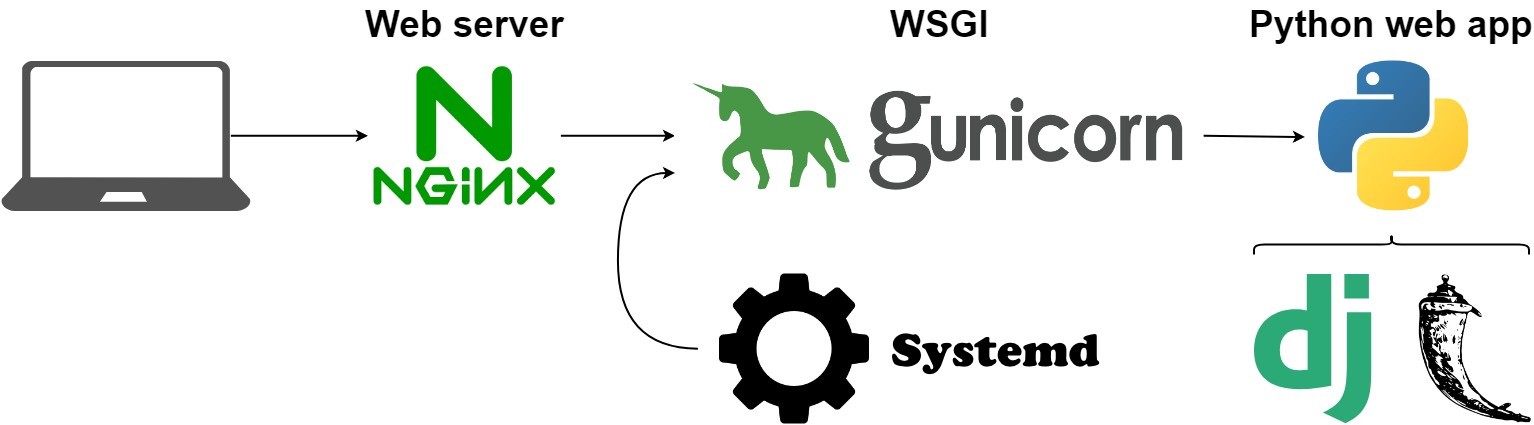
\includegraphics[width=\linewidth]{fig/gunicorn.jpeg}
        \caption{Nginx + Gunicorn + Systemd + Django}
        \label{fig:gunicorn}
    \end{figure}
    Comme montré en Figure \ref{fig:gunicorn}, nous allons utiliser Gunicorn en tant que \emph{service systemd}, ce qui permettra, entre autre, le démarrage automatique du serveur.

    \newpage

        \subsection{Gunicorn}
        Pour commencer, nous devons créer deux fichiers pour interfacer systemd à Gunicorn, \verb|gunicorn.socket| et \verb|gunicorn.service|.
        \begin{listing}[H]
            \begin{minted}{bash}
[Unit]
Description=gunicorn socket
[Socket]
ListenStream=/run/gunicorn.sock
[Install]
WantedBy=sockets.target
            \end{minted}
            \caption{/etc/systemd/system/gunicorn.socket}
            \label{code:gunicorn.socket}
        \end{listing}
        Ce fichier permet de créer un \emph{socket} (ou une \emph{interface de connexion}), qui est, pour faire simple, un moyen que plusieurs applications peuvent utiliser pour communiquer.
        Nous allons utiliser cela pour connecter Gunicorn à Nginx.
        \begin{listing}[H]
            \begin{minted}[breaklines]{bash}
[Unit]
Description=gunicorn daemon
Requires=gunicorn.socket
After=network.target
[Service]
User=toto
Group=www-data
WorkingDirectory=/home/toto/django
ExecStart=/home/toto/django/.venv/bin/gunicorn --access-logfile - --workers 3 --bind unix:/run/gunicorn.sock SAE23.wsgi:application
[Install]
WantedBy=multi-user.target
            \end{minted}
            \caption{/etc/systemd/system/gunicorn.service}
            \label{code:gunicorn.service} 
        \end{listing}
        La création du service nous permet de lancer Gunicorn sous la forme d'un \emph{daemon}.
        Dans ce fichier, nous précisons l'utilisateur et le groupe avec lesquels le service doit être exécuté ainsi que le service doit être exécuté après l'initialisation du réseau.
        Nous pouvons maintenant activer Gunicorn au démarrage.
        \begin{listing}[H]
            \begin{minted}[breaklines]{bash}
systemctl start gunicorn.socket
systemctl enable gunicorn.socket
            \end{minted}
            \caption{Activation du socket Gunicorn}
            \label{code:enable-gunicorn} 
        \end{listing}

        \subsection{Nginx}
        Une fois Gunicorn correctement paramétré, nous pouvons configurer Nginx pour rediriger les connexions sur le socket. Pour cela il faut créer un fichier \emph{site} en suivant la bonne syntaxe.
        \begin{listing}[H]
            \begin{minted}[breaklines]{bash}
server {
    listen 80;
    server_name sae23.louis.systems;
    location = /favicon.ico { access_log off; log_not_found off; }
    location /static/ {
        root /home/toto/django;
    }
    location / {
        include proxy_params;
        proxy_pass http://unix:/run/gunicorn.sock;
    }
}
            \end{minted}
            \caption{/etc/nginx/sites-available/sae23}
            \label{code:sae23-site} 
        \end{listing}
        Pour cet exemple, Nginx écoute sur le port 80 et si un client se connecte en utilisant le domaine \verb|sae23.louis.systems|
        \footnote{Il s'agit du domaine d'un VPS utilisé pour tester le déploiement, car nous n'avons pas réussi à utiliser les cartes bridges sans les droits d'administrateur sur les PC fixes},
        il redirige /static vers le répertoire précédemment configuré, le reste est redirigé vers le socket Gunicorn.
        Une fois ce fichier crée, nous devons l'activer avec un lien symbolique.
        \begin{listing}[H]
            \begin{minted}[breaklines]{bash}
ln -s /etc/nginx/sites-available/sae23 /etc/nginx/sites-enabled/
            \end{minted}
            \caption{Activation du site Nginx}
            \label{code:nginx-site-active} 
        \end{listing}
        Pour finir, nous pouvons redémarrer le service Nginx avec systemd pour prendre en compte les changements.
        \begin{listing}[H]
            \begin{minted}[breaklines]{bash}
systemctl restart nginx
            \end{minted}
            \caption{Redémarrage du service Nginx}
            \label{code:nginx-restart} 
        \end{listing}
    
\section{Script de déploiement automatique}
    Pour faciliter le déploiement, nous avons écrit un simple script bash permettant d'automatiser toutes les étapes de cette procédure dans une VM de Debian 11 fraîchement installée avec un accès root
    \footnote{Le script crée un utilisateur "toto", il est donc préférable que celui-ci n'existe pas déjà}.
    Pour utiliser ce script, nous pouvons simplement utiliser \verb|curl|\footnote{Il est normalement préférable pour la sécurité de lire un script avant de l'exécuter} pour le télécharger directement de GitHub.
    \begin{listing}[H]
        \begin{minted}[breaklines]{bash}
apt install curl
curl -sSL https://raw.githubusercontent.com/ldsvrn/SAE23-TraficAerien/main/server_install.sh | bash
        \end{minted}
        \caption{Exécution du script de déploiement automatique}
        \label{code:script-curl} 
    \end{listing}
    Une fois le script exécuté, il est normalement possible d'accéder au serveur.
    Malheureusement, le script n'est pas interactif, il n'est donc pas universel, en effet, certains détails tels que le \verb|ALLOWED_HOSTS| de Django ou le \verb|server_name| de Nginx nécessitent d'être modifiés en fonction de l'adresse du serveur. Une solution serait de créer une image Docker du projet.
\end{document}